\documentclass[11pt,a4paper]{article}

\usepackage[utf8]{inputenc}
\usepackage[T1]{fontenc}
\usepackage[spanish,es-noshorthands,es-tabla]{babel}
\usepackage{lmodern}
\usepackage[margin=2.5cm]{geometry}
\usepackage{amsmath}
\usepackage{booktabs}
\usepackage{graphicx}
\usepackage{float}
\usepackage{caption}
\usepackage{enumitem}
\usepackage[hidelinks]{hyperref}

\graphicspath{{../benchmark/results/}}
\setlist{itemsep=2pt}

\title{Tarea 1: Escape de la Torre\\[4pt]\large Inteligencia Artificial}
\author{Benjamin Jimenez}
\date{Septiembre 2026}

\begin{document}

\maketitle

\begin{abstract}
Se simula la evacuación de un piso de una torre en llamas y se comparan cinco algoritmos de navegación: dos de búsqueda no informada (BFS, UCS), dos de búsqueda informada (A*, Greedy Best-First) y un algoritmo genético. El entorno es dinámico: el fuego avanza de forma irreversible, las celdas tienen capacidad limitada y los agentes replanifican sus rutas. Sobre 3000 simulaciones (3 mapas, 5 algoritmos, 200 iteraciones, 80 agentes), la supervivencia queda limitada principalmente por el cuello de botella de la salida y por el tiempo que tarda el fuego en rodearla. La única diferencia estadísticamente clara entre algoritmos es la ventaja de A* sobre Greedy en el mapa de pasillos angostos.
\end{abstract}

\section{Introducción}

El objetivo es implementar el sistema de navegación de un grupo de agentes que debe alcanzar la única salida de un piso antes de ser alcanzado por el fuego, minimizando las bajas y mitigando la congestión. Se implementan tres paradigmas: búsqueda no informada, búsqueda informada con heurística admisible y optimización bioinspirada. El desempeño se evalúa mediante un benchmark comparativo de 200 iteraciones por combinación de mapa y algoritmo.

\section{Descripción del entorno}

\subsection{Grilla y mapas}

El espacio se discretiza en una grilla regular cuyas celdas pueden ser libres, muros, fuego o salida. Cada piso tiene una única salida.

\begin{itemize}
  \item \textbf{Mapa 1} ($7\times7$, alta densidad / cuello de botella): pasillos angostos que convergen hacia la salida.
  \item \textbf{Mapa 2} ($8\times8$, densidad media / laberinto corporativo): salas conectadas por intersecciones y cruces ciegos.
  \item \textbf{Mapa 3} ($9\times9$, baja densidad / dispersión abierta): entorno semiabierto con varias rutas alternativas.
\end{itemize}

\subsection{Congestión: costo y capacidad}

La congestión se modela en dos niveles.

\paragraph{Costo de planificación.} Entrar a una celda $c$ cuesta
\begin{equation}
  \text{costo}(c) = 1 + k \cdot \text{ocupación}(c)^2, \qquad k = 0.1,
\end{equation}
un modelo cuadrático que penaliza fuertemente las celdas con varios agentes. UCS, A* y el algoritmo genético usan este costo; BFS y Greedy no.

\paragraph{Capacidad física.} Cada celda admite como máximo 3 agentes simultáneos. Si la celda siguiente de la ruta está llena, el agente espera en su lugar. En la salida, los agentes evacuados se retiran al final del turno, por lo que evacúan como máximo 3 agentes por turno. Esto reproduce el embotellamiento que retrasa el flujo.

\subsection{Propagación del fuego}

Cada mapa tiene dos focos fijos. Además, en cada iteración se enciende al azar cerca del 5\% de las celdas libres según la semilla, cuidando que la salida siga conectada. Cada $k=3$ turnos el fuego se expande a las celdas ortogonales adyacentes. Las celdas quemadas quedan intransitables para el resto de la simulación y la salida está protegida. Un agente alcanzado por el fuego es una baja.

\subsection{Movimiento y replanificación}

Los agentes solo se desplazan en forma ortogonal (arriba, abajo, izquierda, derecha) o esperan. Cualquier paso que no sea a una celda vecina transitable se rechaza. Cada vez que el fuego se propaga, todos los agentes vivos recalculan su ruta con el algoritmo en evaluación, considerando la ocupación actual.

\subsection{Orden de un turno}

\begin{enumerate}
  \item Cada agente vivo intenta avanzar un paso de su ruta, o espera si la celda está llena.
  \item Los agentes que llegaron a la salida se retiran del entorno.
  \item El fuego avanza (cada 3 turnos) y los agentes en celdas quemadas mueren.
  \item Si el fuego avanzó, los agentes replanifican.
\end{enumerate}

\section{Algoritmos implementados}

\subsection{Búsqueda no informada}

\paragraph{BFS (Breadth-First Search).} Expande nodos por niveles con una cola FIFO y un conjunto de visitados. Encuentra la ruta con menos pasos, pero ignora la congestión. Sirve como línea base.

\paragraph{UCS (Uniform Cost Search).} Expande el nodo de menor costo acumulado con una cola de prioridad. Como el costo de cada celda incluye la congestión, encuentra la ruta de menor costo total según la ocupación al momento de planificar.

\subsection{Búsqueda informada}

\paragraph{A*.} Ordena la frontera por $f(n) = g(n) + h(n)$, donde $g(n)$ es el costo acumulado con congestión y $h(n)$ la distancia Manhattan a la salida:
\begin{equation}
  h(n) = |r_n - r_s| + |c_n - c_s|.
\end{equation}
La heurística es admisible: con movimiento ortogonal cada paso cuesta al menos 1, así que nunca sobreestima el costo real. Por lo tanto, A* es óptimo respecto del costo.

\paragraph{Greedy Best-First.} Ordena la frontera solo por $h(n)$, sin costo acumulado. Explora menos nodos, pero no es óptimo y no considera la congestión.

\subsection{Optimización bioinspirada: algoritmo genético}

\begin{itemize}
  \item \textbf{Individuo:} secuencia de acciones (arriba, abajo, izquierda, derecha, esperar). Se decodifica desde la posición del agente; una acción que choca con un muro, el fuego o el borde se interpreta como esperar. Así, toda ruta generada respeta el movimiento ortogonal de una casilla.
  \item \textbf{Población inicial:} 15 individuos; 60\% sembrados con la ruta de A* (convertida a acciones, más una cola aleatoria de hasta 5 acciones) y 40\% aleatorios, con longitud entre 20 y 150.
  \item \textbf{Fitness:}
  \begin{equation}
    F =
    \begin{cases}
      200 - \text{pasos} - 0.05 \cdot \text{costo} & \text{si la ruta llega a la salida},\\
      -\,d_{\text{Manhattan}} - 2 \cdot \text{costo} & \text{si no llega}.
    \end{cases}
  \end{equation}
  \item \textbf{Selección:} torneo de tamaño 3.
  \item \textbf{Cruce:} un punto de corte.
  \item \textbf{Mutación:} cada gen se reemplaza por una acción aleatoria con probabilidad 0.2.
  \item \textbf{Elitismo:} se conserva el 20\% mejor de cada generación.
  \item \textbf{Generaciones:} 20. Se ejecuta al inicio y en cada replanificación.
\end{itemize}

\section{Resultados experimentales}

\subsection{Configuración del benchmark}

\begin{itemize}
  \item 3 mapas $\times$ 5 algoritmos $\times$ 200 iteraciones = 3000 simulaciones, con 80 agentes cada una.
  \item Cada iteración usa una semilla aleatoria distinta, que determina el fuego inicial y las posiciones de los agentes.
  \item $k = 0.1$ (congestión), capacidad 3 por celda, propagación cada 3 turnos, máximo 500 turnos.
\end{itemize}

\paragraph{Métricas.}
\begin{itemize}
  \item \textbf{Tasa de supervivencia:} $N_{\text{sobrevivientes}} / N_{\text{total}}$ por simulación, promediada sobre las 200 iteraciones. Se reporta el intervalo de confianza del 95\% de la media, $\bar{x} \pm 1.96\,\sigma/\sqrt{n}$.
  \item \textbf{Tiempo de despeje:} turno en que el último sobreviviente alcanza la salida. Se reportan media, desviación estándar, mínimo y máximo.
\end{itemize}

\subsection{Tabla de resultados}

\begin{table}[H]
\centering
\caption{Resultados del benchmark (200 iteraciones por fila, 80 agentes).}
\label{tab:resultados}
\begin{tabular}{llcrrrr}
\toprule
Mapa & Algoritmo & Supervivencia (IC 95\%) & Media & Std & Mín & Máx \\
\midrule
map1 & BFS     & 0.545 [0.508, 0.582] & 16.93 & 8.23 & 1 & 28 \\
map1 & UCS     & 0.558 [0.522, 0.593] & 17.25 & 7.94 & 1 & 28 \\
map1 & A*      & \textbf{0.583} [0.549, 0.616] & 17.91 & 7.54 & 4 & 28 \\
map1 & Greedy  & 0.515 [0.477, 0.552] & 15.86 & 8.37 & 2 & 28 \\
map1 & Genético & 0.559 [0.525, 0.594] & 17.23 & 7.74 & 1 & 28 \\
\midrule
map2 & BFS     & 0.424 [0.411, 0.438] & 12.23 & 2.32 & 3 & 14 \\
map2 & UCS     & 0.425 [0.413, 0.437] & 12.29 & 2.06 & 2 & 14 \\
map2 & A*      & \textbf{0.427} [0.415, 0.438] & 12.30 & 1.89 & 1 & 14 \\
map2 & Greedy  & 0.415 [0.403, 0.427] & 12.13 & 2.03 & 2 & 14 \\
map2 & Genético & 0.424 [0.412, 0.436] & 12.31 & 2.06 & 1 & 14 \\
\midrule
map3 & BFS     & 0.364 [0.347, 0.382] & 10.79 & 3.54 & 3 & 15 \\
map3 & UCS     & 0.347 [0.330, 0.365] & 10.24 & 3.41 & 2 & 15 \\
map3 & A*      & 0.348 [0.331, 0.366] & 10.27 & 3.49 & 1 & 15 \\
map3 & Greedy  & 0.349 [0.331, 0.367] & 10.44 & 3.45 & 3 & 15 \\
map3 & Genético & \textbf{0.371} [0.354, 0.388] & 10.91 & 3.37 & 1 & 15 \\
\bottomrule
\end{tabular}

\smallskip
\footnotesize Media, Std, Mín y Máx corresponden al tiempo de despeje en turnos.
\end{table}

\begin{figure}[H]
  \centering
  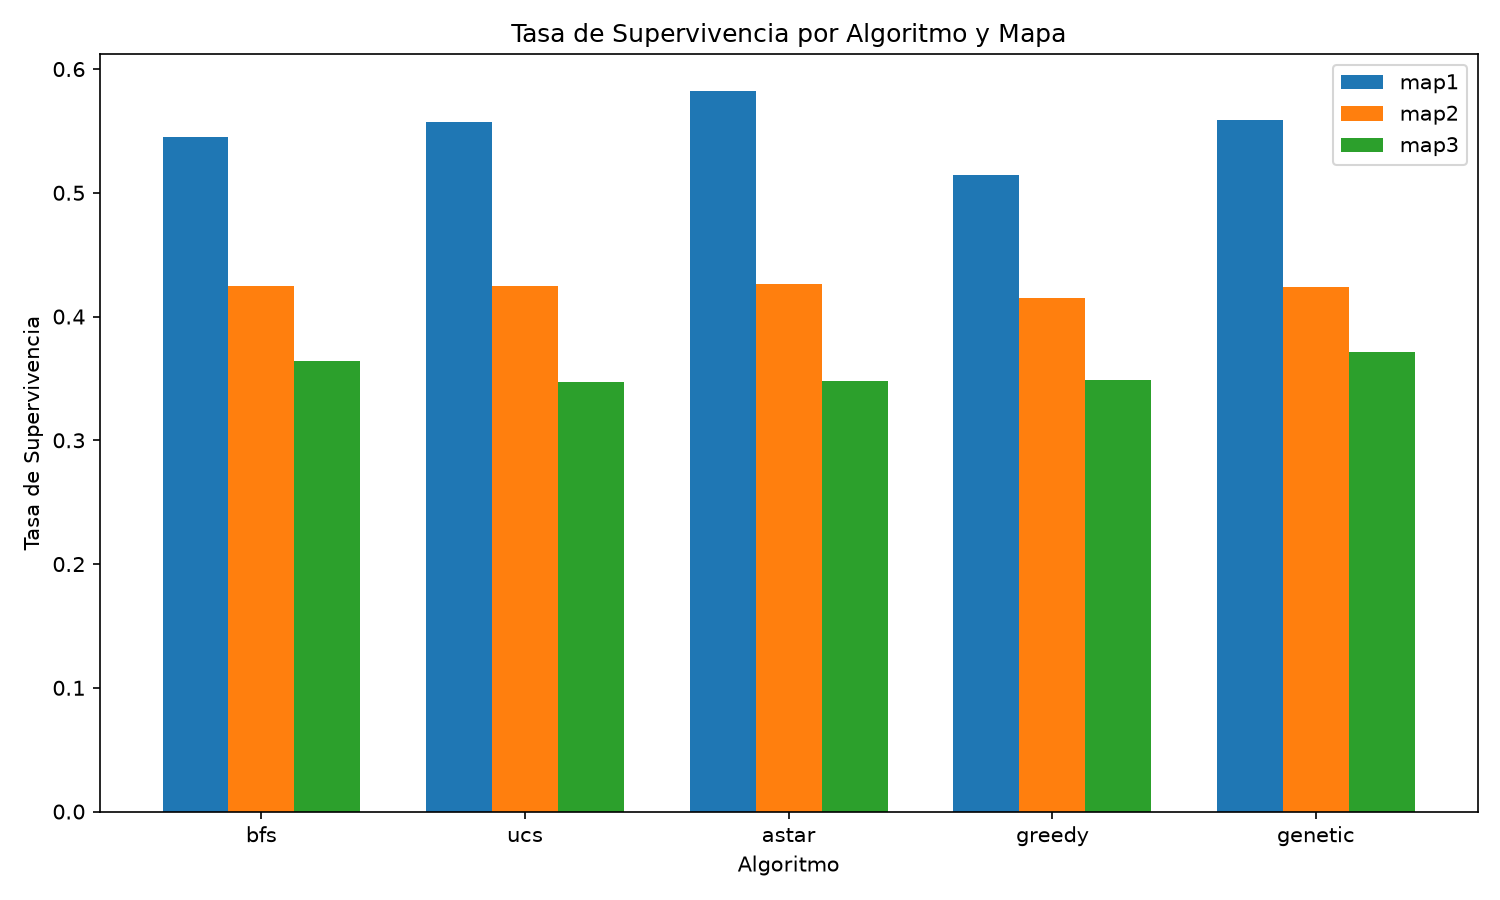
\includegraphics[width=0.85\textwidth]{tasa_supervivencia.png}
  \caption{Tasa de supervivencia media por algoritmo y mapa.}
  \label{fig:supervivencia}
\end{figure}

\begin{figure}[H]
  \centering
  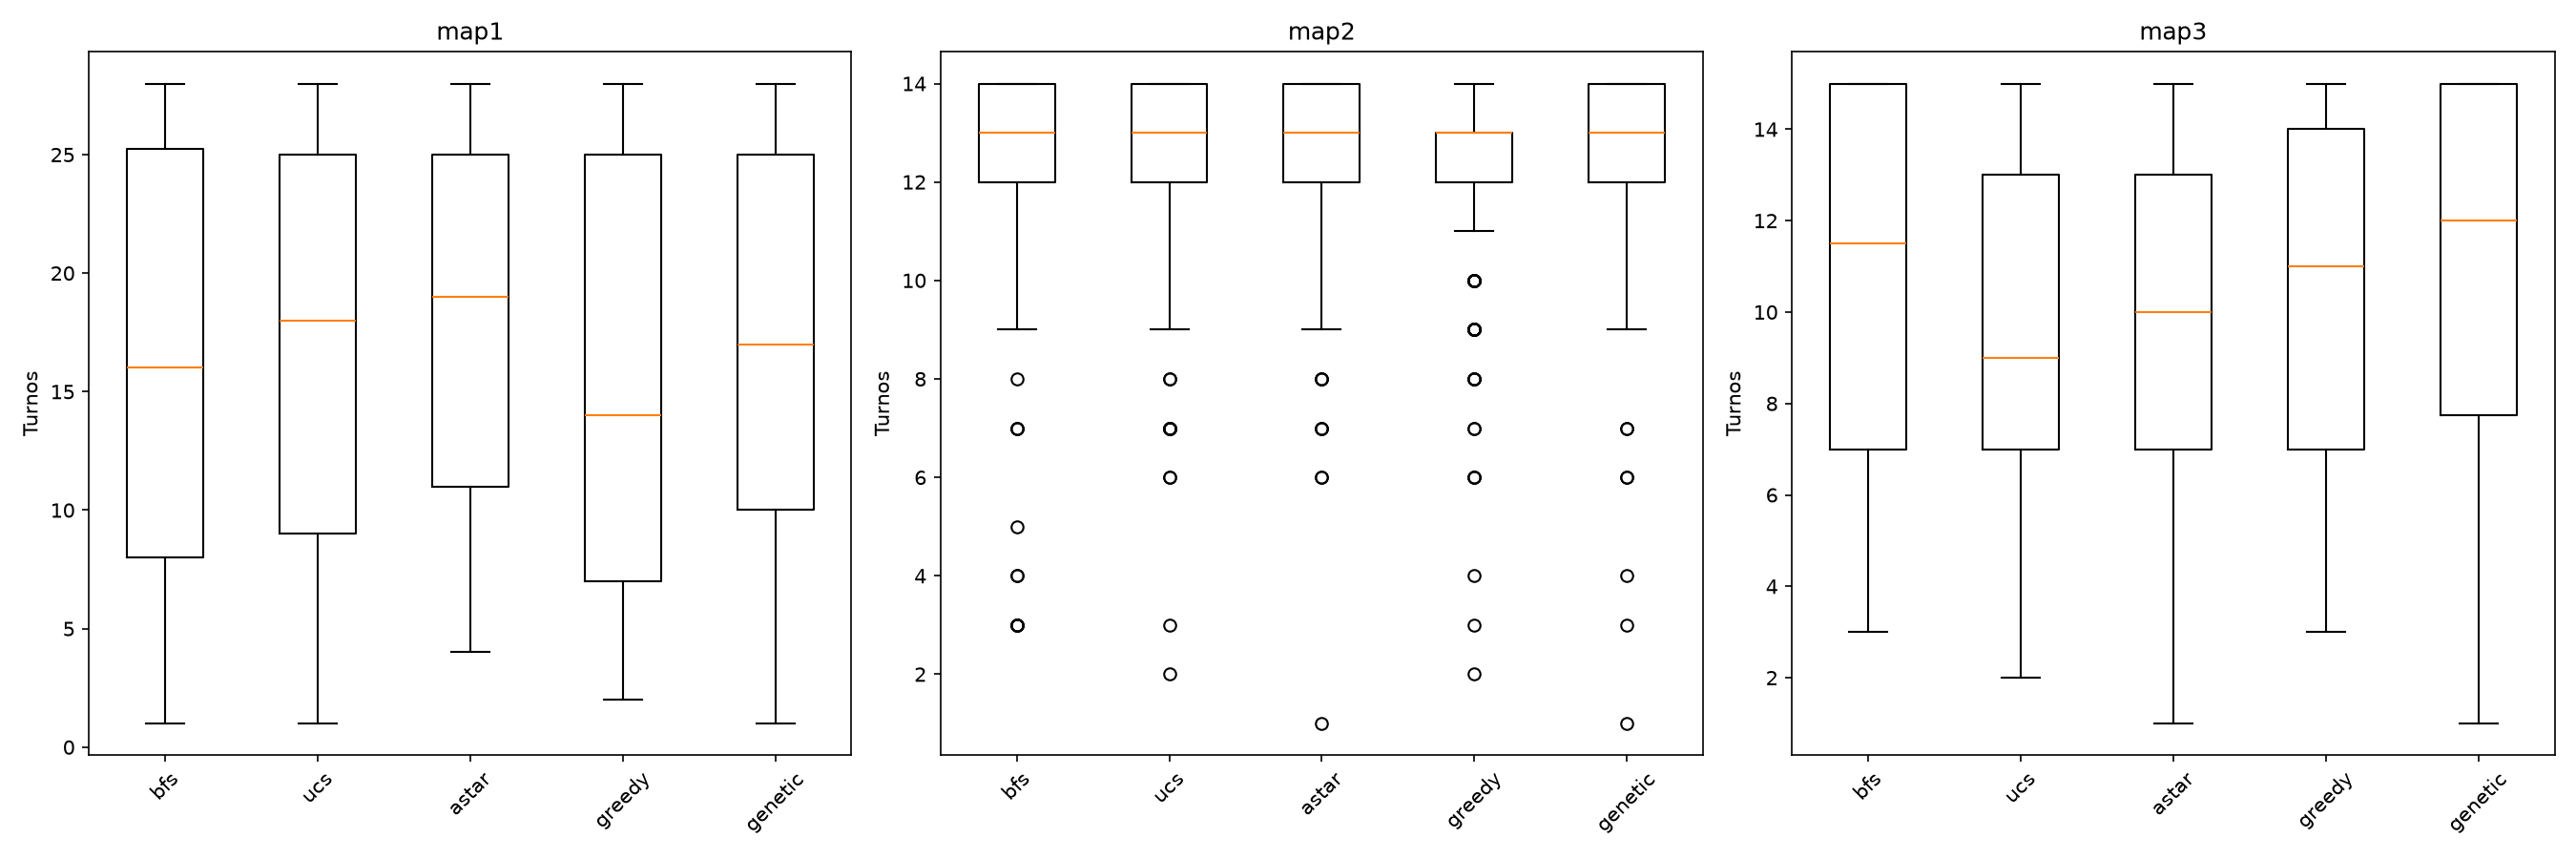
\includegraphics[width=\textwidth]{boxplot_turnos_por_algoritmo.png}
  \caption{Distribución del tiempo de despeje (turnos) por algoritmo en cada mapa.}
  \label{fig:boxplot}
\end{figure}

\begin{figure}[H]
  \centering
  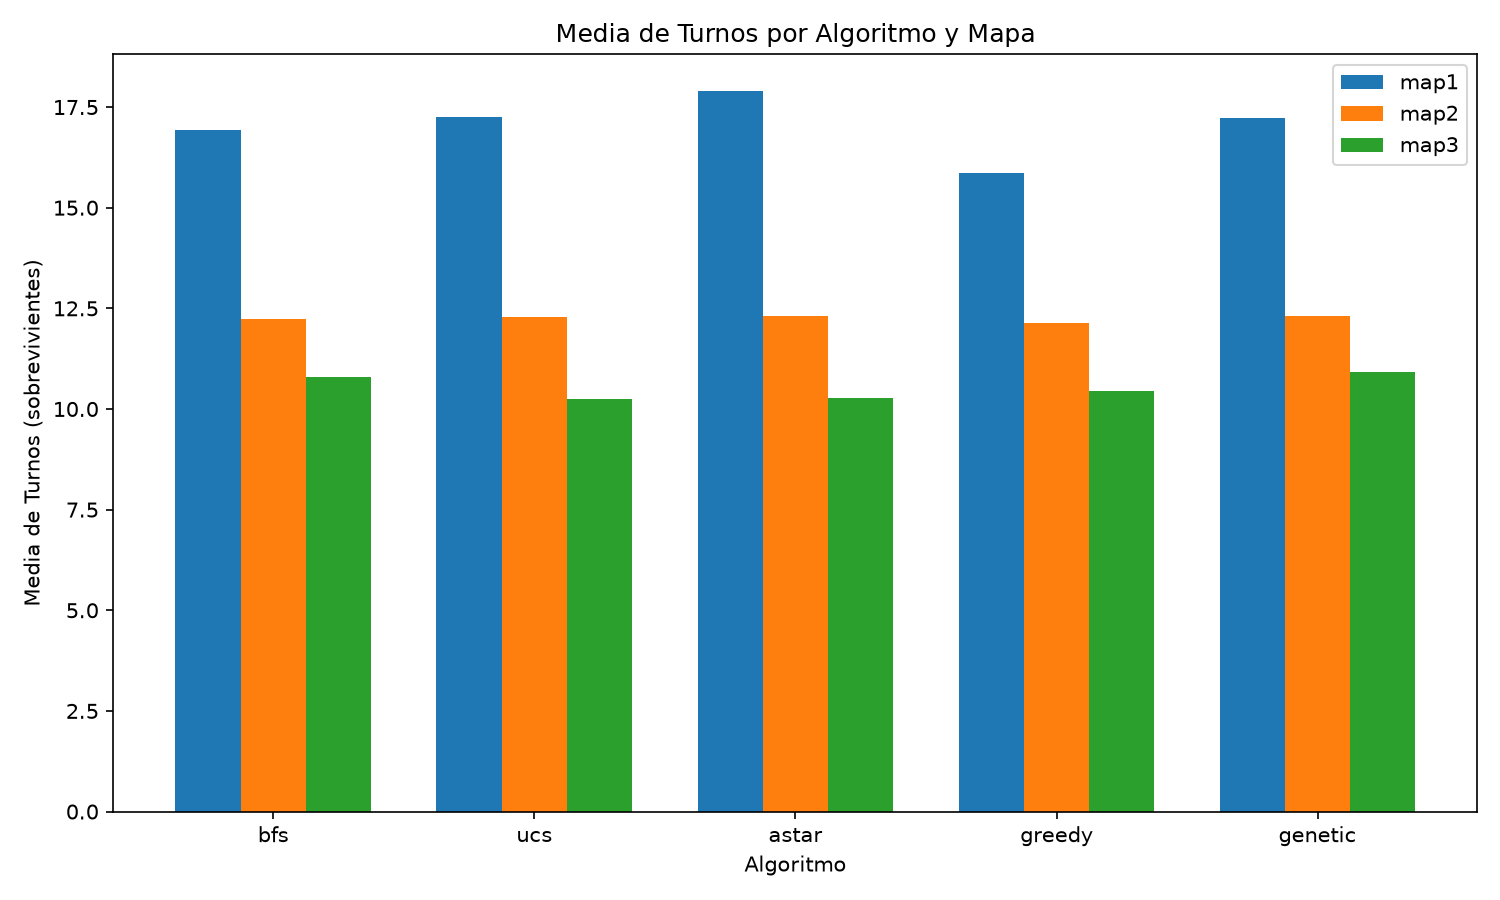
\includegraphics[width=0.85\textwidth]{media_turnos.png}
  \caption{Tiempo de despeje medio por algoritmo y mapa.}
  \label{fig:media}
\end{figure}

\subsection{Análisis: el cuello de botella de la salida}

El resultado central es que la supervivencia queda limitada principalmente por el entorno y no por el algoritmo. Dos mecanismos lo explican.

\paragraph{Capacidad de la salida.} Como solo evacúan 3 agentes por turno, el número de sobrevivientes no puede superar $3T$, donde $T$ es el tiempo de despeje. En promedio, los agentes evacuados alcanzan entre el 86\% y el 91\% de esa cota: la salida trabaja casi siempre a plena capacidad.

\paragraph{Sellado de la salida por el fuego.} Aunque la celda de salida está protegida, el fuego termina ocupando todas sus celdas vecinas. Esto ocurrió en el 100\% de las semillas, en promedio en el turno 29.7 (mapa 1), 14.2 (mapa 2) y 11.3 (mapa 3). Por eso el máximo de turnos es idéntico para todos los algoritmos (28, 14 y 15).

Con la salida saturada y un tiempo disponible fijado por el fuego, cualquier algoritmo que lleve agentes a la salida de forma continua obtiene una supervivencia similar.

\subsection{Análisis por algoritmo}

\begin{itemize}
  \item \textbf{A*} obtiene la mayor supervivencia en el mapa 1 (0.583) y es el único caso con diferencia estadísticamente clara: su IC 95\% no se solapa con el de Greedy (0.515). Al sumar el costo de congestión a la heurística, reparte mejor a los agentes en los pasillos angostos.
  \item \textbf{Greedy} tiene la menor supervivencia en los mapas 1 y 2. Al ignorar el costo acumulado, probablemente concentra más agentes en las mismas celdas.
  \item \textbf{BFS y UCS} quedan en posiciones intermedias. UCS no supera claramente a BFS: la congestión solo se conoce al planificar y cambia en cuanto los agentes se mueven.
  \item \textbf{El algoritmo genético} rinde a la par de los métodos de búsqueda (el mejor valor en el mapa 3, 0.371, dentro del margen de error de BFS). Su siembra con A* le entrega rutas válidas desde el inicio y, con 15 individuos y 20 generaciones, la evolución las modifica poco. Es además el más costoso computacionalmente: cerca de 3\,s por simulación, frente a menos de 0.1\,s de los demás.
\end{itemize}

\subsection{Análisis por mapa}

\begin{itemize}
  \item \textbf{Mapa 1} (cuello de botella): mayor supervivencia (0.52--0.58) y mayor variabilidad (desviación de unos 8 turnos), porque el fuego tarda más en sellar la salida y ese tiempo varía mucho según la semilla. Es el único mapa donde el algoritmo marca una diferencia.
  \item \textbf{Mapa 2} (laberinto): supervivencia cercana a 0.42 para todos, con muy poca dispersión. La salida se sella cerca del turno 14 en casi todas las semillas, lo que limita la evacuación a unos 42 agentes ($3 \times 14$).
  \item \textbf{Mapa 3} (abierto): la menor supervivencia (0.35--0.37), pese a ser el mapa con más rutas. Uno de los focos iniciales está en la misma fila que la salida y la alcanza rápido: la posición del fuego respecto de la salida pesa más que la densidad de muros.
\end{itemize}

\section{Conclusiones}

\begin{itemize}
  \item Con 80 agentes y una salida de capacidad 3, el cuello de botella común domina el resultado: la supervivencia depende sobre todo de cuánto tarda el fuego en sellar la salida.
  \item A* es el algoritmo más robusto: tiene la mejor supervivencia en el único mapa con diferencias significativas y en los demás no es significativamente peor que ningún otro.
  \item Greedy es el más débil cuando hay congestión, porque no considera el costo del camino.
  \item El algoritmo genético es competitivo, pero no mejora a A*, del que depende su población inicial, y su costo computacional es mucho mayor.
  \item Para que el benchmark distinga mejor a los algoritmos se necesitaría más holgura temporal: más distancia entre el fuego y la salida, mapas más grandes o menos agentes en relación con la capacidad de la salida.
\end{itemize}

\subsection{Limitaciones}

\begin{itemize}
  \item La congestión que ven los algoritmos es la del instante de planificación; los agentes no se coordinan ni reservan celdas.
  \item Los agentes esperan solo cuando la celda siguiente está llena; la acción de esperar no forma parte del espacio de búsqueda de BFS, UCS, A* ni Greedy (sí del algoritmo genético).
  \item Cada algoritmo se evaluó con semillas aleatorias independientes; usar las mismas 200 semillas para todos permitiría comparaciones pareadas.
\end{itemize}

\subsection{Trabajo futuro}

\begin{itemize}
  \item Planificación cooperativa con reserva de celdas en el tiempo (por ejemplo, Cooperative A*).
  \item Incluir la acción de esperar y la predicción del avance del fuego en la búsqueda.
  \item Heurísticas que consideren la distancia al frente de fuego.
  \item Escenarios con más holgura temporal para diferenciar mejor los algoritmos.
  \item Visualización gráfica del entorno multiagente.
\end{itemize}

\section{Fuentes y uso de IA generativa}

\begin{itemize}
  \item Russell, S. y Norvig, P. (2020). \emph{Artificial Intelligence: A Modern Approach} (4.ª ed.). Pearson. --- BFS, UCS, A*, Greedy Best-First.
  \item Goldberg, D. E. (1989). \emph{Genetic Algorithms in Search, Optimization, and Machine Learning}. Addison-Wesley. --- Algoritmo genético.
  \item La heurística Manhattan es un concepto estándar de inteligencia artificial.
  \item No se utilizaron repositorios externos para los algoritmos de búsqueda.
\end{itemize}

\paragraph{Uso de IA generativa.} Se utilizó Claude Code (Anthropic) como asistente para corregir errores del entorno y la simulación (capacidad por celda, conteo de ocupación, métrica de tiempo de despeje), para reescribir la representación del algoritmo genético como secuencia de acciones y para redactar este informe a partir de los resultados del benchmark.

\end{document}
